\subsubsection{Trapezoidal rule}

\textbf{Idea:} Use trapezoids to approximate the area under the graph.

\begin{figure*}[h]
    \centering
    \includegraphics[width=0.5\textwidth]{trapezoid}
\end{figure*}

Let $P$ be a partition with $x_i,\ i = 0,\dots, n;\ x_0 = a,\ x_n = b$.
In each subinterval the integral is approximated by:
\[
    \int_{x_i}^{x_{i+1}} f(x) \,dx \approx
    (x_{i+1} - x_i) \cdot \frac{f(x_{i+1}) + f(x_i)}{2}
\]
Here we are multiplying the width of the base by the average height of the trapezoid.

Summing over all sub-intervals:
\[
    T(f; P) = \frac{1}{2} \sum_{i=0}^{n-1} (x_{i+1} - x_i) \bigl(f(x_{i+1}) + f(x_i)\bigr)
\]
If pratition is equidistant, i.e. $x_{i+1} - x_i = h$:
\[
    T(f; P) = \frac{h}{2} \sum_{i=0}^{n-1} \bigl(f(x_{i+1}) + f(x_i)\bigr) =
    h \sum_{i=1}^{n-2} f(x_i) + \frac{h}{2} \bigl(f(x_0) + f(x_n)\bigr)
\]
\begin{theorem}
    Let $f \in C^2([a, b])$ and $P$ an equidistant partition of $[a, b]$.
    Then, the error of the trapezoidal rule is:
    \begin{align*}
        &\abs{\int_a^b f(x)\,dx - T(f; P)} = 
        \frac{1}{12} \abs{(b - a) h^2 f''(\xi)}
        \\&
        \xi \in (a, b),\ h = x_{i+1} - x_i
    \end{align*}
\end{theorem}
\begin{proof}
    Can be done by applying integration by parts twice, or by using linear interpolation.
\end{proof}
\begin{consequence}
    The error of equidistant trapezoidal rule is order $\mathcal{O}(h^2)$.
\end{consequence}

It is particularly interesting to use the trapezoidal rule for 
$n = 2^m$, i.e. $2, 4, 8, 16, \dots$ sub-intervals.
For these partitions it is possible to derive a recursive trapezoidal rule:
\[
    T_m(f; P) = \frac{1}{2} T_{m-1}(f; P) + 
    h \sum_{i=1}^{2^{m-1}} f(a + (2i - 1) h)
    \text{ for } m \ge 1,\ h = \frac{b - a}{2^m}
\]
This can be used for iteratively refining the approximation result.

\subsubsection{Romberg Algorithm}
\textbf{Idea:} Use trapezoidal rule and Richardson extrapolation.
\begin{enumerate}
    \item {
        Use trapezoidal rule for sequence of partitions
        $n = 2^0, 2^1, 2^2, \dots, 2^m,\ m \in \mathbb{N}$.
        This yields approximation of integral
        \[ R_i^0 \coloneqq T_i(f; P) \]
        That's the trapezoidal rule for $2^i$ subintervals, i.e.
        \[ h = \frac{b - a}{2^i} \]
        These numbers yield the first column in the Romberg array:
        \begin{center}
            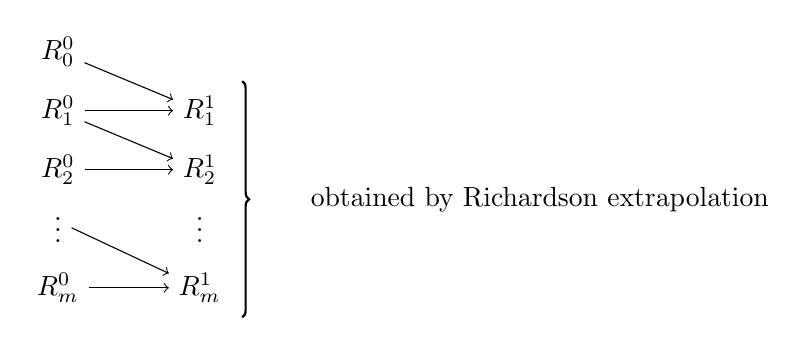
\begin{tikzpicture}[x=1.8cm,y=0.75cm]
                \node[] at (0, 0) (00) {$R^0_0$};
                \node[] at (0, -1) (01) {$R^0_1$};
                \node[] at (0, -2) (02) {$R^0_2$};
                \node[] at (0, -2.875) (03) {$\vdots$};
                \node[] at (0, -4) (04) {$R^0_m$};
                \node[] at (1, -1) (11) {$R^1_1$};
                \node[] at (1, -2) (12) {$R^1_2$};
                \node[] at (1, -2.875) (13) {$\vdots$};
                \node[] at (1, -4) (14) {$R^1_m$};
        
                \draw [->] (00) -- (11);
                \draw [->] (01) -- (11);
                \draw [->] (01) -- (12);
                \draw [->] (02) -- (12);
                \draw [->] (03) -- (14);
                \draw [->] (04) -- (14);

                \draw [thick, decorate, decoration = {brace}] (1.3,-0.5) -- (1.3,-4.5);
                \node[] at (3.4, -2.5) () {obtained by Richardson extrapolation};
            \end{tikzpicture}
        \end{center}
    }
    \item {
        Write down error in Taylor series expansion.

        Trapezoidal rule for $i - 1$ sub-intervals.
        \[
            \int_a^b f(x) \,dx = R_{i-1}^0 + a_2 h^2 + a_4 h^4 + a_6 h^6 + \ldots = \text{(1)}
        \]
        Note that only even powers appear.

        (We're not going to prove this formula. For the proof, one
        can write the Taylor series of $f$ for a point on each the subintervals of length $h$ in the trapezoidal rule,
        then integrate each of those Taylor series and sum them up.)

        Trapezoidal rule for $i$ sub-intervals:
        \[
            \int_a^b f(x) \,dx = R_{i}^0 + a_2 \Bigl(\frac{h}{2}\Bigr)^2 + 
            a_4 \Bigl(\frac{h}{2}\Bigr)^4 + a_6 \Bigl(\frac{h}{2}\Bigr)^6 + \ldots = 
            R_i^0 + \frac{a_2}{4} h^2 + \frac{a_4}{16} h^4 + \frac{a_6}{64} h^6
            = \text{(2)}
        \]
        (No proof here either.)

        Now take $\text{(1)} - 4 \times \text{(2)}$:
        \begin{align*}
            &-3 \int_a^b f(x) \,dx = (R_{i-1}^0 - 4R_i^0) + \frac{3}{4} a_4 h^4 + 
            \frac{15}{16} a_6 h^6 + \dots
            \\& \iff 
            \int_a^b f(x) \,dx = \Bigl(\frac{R_{i-1} - 4R_i^0}{-3}\Bigr) - 
            \frac{a_4}{4} h^4 - \frac{5}{16} a_6 h^6 - \ldots = 
            R_i^1 - \mathcal{O}(h^4)
        \end{align*}
        So,
        \[R_i^1 = \frac{4}{3} R_i^0 - \frac{1}{3} R_{i-1}^0 \]
        is a better approximation.

        Repeat this process to yield a second column in the Romberg array.
        Further columns ($R^2 \dots R^m$) are produced by Richardson extrapolation.
        \begin{center}
            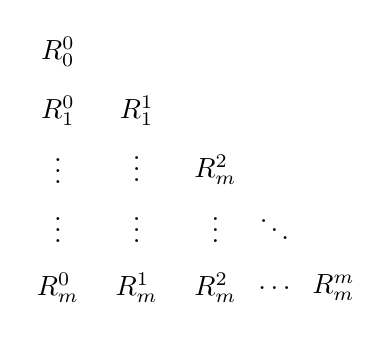
\begin{tikzpicture}[x=1cm,y=0.75cm]
                \node[] at (0, 0) (00) {$R^0_0$};
                \node[] at (0, -1) (01) {$R^0_1$};
                \node[] at (0, -1.875) (02) {$\vdots$};
                \node[] at (0, -2.875) (03) {$\vdots$};
                \node[] at (0, -4) (04) {$R^0_m$};
                \node[] at (1, -1) (11) {$R^1_1$};
                \node[] at (1, -1.85) (12) {$\vdots$};
                \node[] at (1, -2.875) (13) {$\vdots$};
                \node[] at (1, -4) (14) {$R^1_m$};
                \node[] at (2, -2) (22) {$R^2_m$};
                \node[] at (2, -2.875) (23) {$\vdots$};
                \node[] at (2, -4) (24) {$R^2_m$};
                \node[] at (2.75, -4) (34) {$\dots$};
                \node[] at (2.75, -2.875) (34) {$\ddots$};
                \node[] at (3.5, -4) (44) {$R^m_m$};
            \end{tikzpicture}
        \end{center}
    }
\end{enumerate}
\begin{example}
    \mbox{}
    \begin{center}   
        \begin{tikzpicture}
            \begin{axis}[
                axis x line=left,
                axis y line=none,
                axis line style={-{}},
                xtick={0, 1},
                xticklabels={$a$, $b$},
                ytick=\empty,
                xmin=0, xmax=1, ymin=0, ymax=1
            ]\end{axis}
        \end{tikzpicture}
    \end{center}
    
    $R_0^0 = T_0(f; P)$, i.e. $2^0 = 1$ subintervals, $h_0 = (b - a)$.

    $R_1^0 = T_1(f; P)$, i.e. $2^1 = 2$ subintervals, $h_1 = \frac{b - a}{2} = \frac{h_0}{2}$.

    $R_2^0 = T_2(f; P)$, i.e. $2^2 = 4$ subintervals, $h_2 = \frac{b - a}{4} = \frac{h_1}{2} = \frac{h_0}{4}$.
    Therefore:
    \begin{align*}
        &R_0^0 = T_0(f; P) = (b - a) \frac{f(b) + f(a)}{2}
        \\&
        R_0^1 = T_1(f;P) = \frac{b-a}{2} \biggl(
            \frac{f\bigl(\frac{b+a}{2}\bigr) + f(a)}{2} +
            \frac{f(b) + f\bigl(\frac{b+a}{2}\bigr)}{2}
        \biggr)
        \text{ --- sum of two trapezoids:}
    \end{align*}
    \begin{center}   
        \begin{tikzpicture}
            \begin{axis}[
                axis x line=left,
                axis y line=left,
                axis line style={-{Stealth[scale=1.5]}},
                xtick={0, 1, 2},
                xticklabels={$a$, $\frac{b+a}{2}$, $b$},
                ytick=\empty,
                xmin=-0.5, xmax=2.5, ymin=0, ymax=1.25,
                unit vector ratio=1 1 1,
                samples=100,
            ]
                \tikzset{graph/.style={very thick, smooth}}

                \addplot[red, graph, domain=0:2] {1 - (x - 1)^2 / 3};
                \addplot[blue, graph,name path=left,domain=0:1] {1 - abs(x - 1) / 3};
                \addplot[blue, graph,name path=right,domain=1:2] {1 - abs(x - 1) / 3};
                \path[name path=axis_left] (axis cs:0,0) -- (axis cs:1,0);
                \path[name path=axis_right] (axis cs:1,0) -- (axis cs:2,0);
                \addplot[pattern color=blue,pattern=north east lines] fill between[of=left and axis_left];
                \addplot[pattern color=blue,pattern=north west lines] fill between[of=right and axis_right];

                \addplot[blue,very thick] coordinates {(0,0) (0,1-1/3)};
                \addplot[blue,very thick] coordinates {(1,0) (1,1)};
                \addplot[blue,very thick] coordinates {(2,0) (2,1-1/3)};
                \addplot[blue,very thick] coordinates {(0,0) (2,0)};
            \end{axis}
        \end{tikzpicture}
    \end{center}
\end{example}

In general we need the following combination:
\[
    R_i^k = R_i^{k-1} + \frac{1}{4^k - 1} (R_i^{k-1} - R_{i-1}^{k-1})
\]

\begin{example}
    If $R_3^2 = 1$ and $R_4^2 = 8$:
    \[
        R_4^3 = R_2^4 + \frac{1}{4^3 - 1} (R_4^2 - R_3^2) =
        8 + \frac{1}{63} (8 - 1) = \frac{73}{9} \approx 8.111\dots
    \]
    In this formula, the value resulting from more intervals ($i$ instead of $i-1$)
    has a greater influence.
\end{example}

\begin{example}
    Apply Romberg Algorithm to find $R_2^2$ for integral
    \[ \int_1^3 \frac{1}{x} \,dx \]
    We can first calculate the integral analytically, to see how well the Romberg algorithm converges:
    \[
        \int_1^3 \frac{1}{x} \,dx = \log(3) - \log(1) = \log(3) \approx 1.09861
    \]
    To start with Romberg we need the trapezoidal rule:
    \begin{center}
        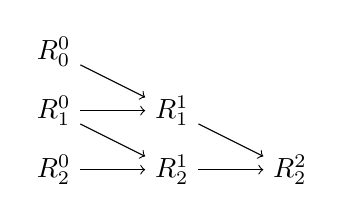
\begin{tikzpicture}[x=1.5cm,y=0.75cm]
            \node[] at (0, 0) (00) {$R^0_0$};
            \node[] at (0, -1) (01) {$R^0_1$};
            \node[] at (0, -2) (02) {$R^0_2$};
            \node[] at (1, -1) (11) {$R^1_1$};
            \node[] at (1, -2) (12) {$R^1_2$};
            \node[] at (2, -2) (22) {$R^2_2$};

            \draw [->] (00) -- (11);
            \draw [->] (01) -- (11);
            \draw [->] (01) -- (12);
            \draw [->] (02) -- (12);
            \draw [->] (11) -- (22);
            \draw [->] (12) -- (22);
        \end{tikzpicture}
    \end{center}
    Now:
    \begin{align*}
        R_0^0 &= (3 - 1) \cdot \frac{1}{2} \Bigl(\frac{1}{1} + \frac{1}{3}\Bigr) = 
        2 \cdot \frac{1}{2} \cdot \frac{4}{3} = \frac{4}{3}
        \\
        R_1^0 &= 1 {\footnotesize\text{ (sub-interval width)}} \biggl(
            \frac{1}{2} \Bigl( \frac{1}{1} + \frac{1}{2} \Bigr){\footnotesize\text{ (1st trap.)}} + 
            \frac{1}{2} \Bigl(\frac{1}{2} + \frac{1}{3} \Bigr){\footnotesize\text{ (2nd trap.)}}
        \biggr)
        \\&= 
        \frac{1}{2} \Bigl(\frac{3}{2} + \frac{5}{6}\Bigr) = \frac{7}{6}
        \\
        R_2^0 &= \frac{1}{2} \cdot \frac{1}{2} \Bigl(
            \frac{1}{1} + \frac{1}{\frac{3}{2}} {\footnotesize\text{ (1st trap.)}} + 
            \frac{1}{\frac{3}{2}} + \frac{1}{2} {\footnotesize\text{ (2nd trap.)}} + 
            \frac{1}{2} + \frac{1}{\frac{5}{2}} {\footnotesize\text{ (3rd trap.)}} + 
            \frac{1}{\frac{5}{2}} + \frac{1}{3} {\footnotesize\text{ (4th trap.)}}
        \Bigr)
        \\&= \frac{1}{4} \Bigl(1 + \frac{4}{3} + 1 + \frac{4}{5} + \frac{1}{3}\Bigr) =
        \frac{67}{60}
    \end{align*}
    Now use the general formula to get the next values in the Romberg array:
    \[
    R_i^k = R_i^{k-1} + \frac{1}{4^k - 1} (R_i^{k-1} - R_{i-1}^{k-1})
    \]
    \begin{center}
        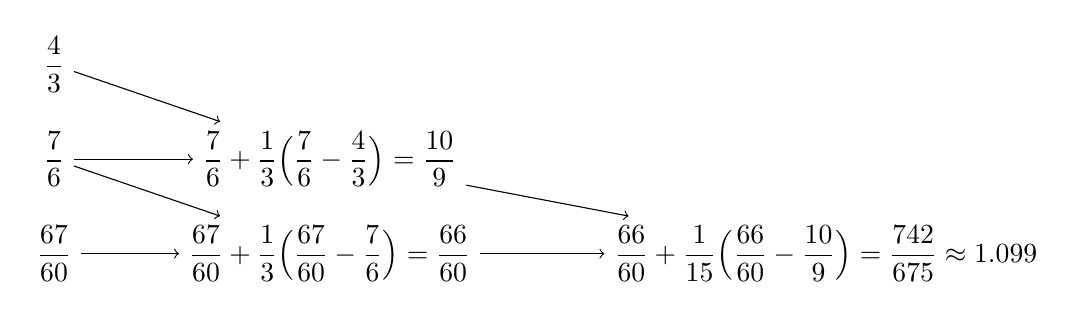
\begin{tikzpicture}[x=3.5cm,y=1.2cm]
            \node[] at (0, 0) (00) {$\displaystyle \frac{4}{3}$};
            \node[] at (0, -1) (01) {$\displaystyle \frac{7}{6}$};
            \node[] at (0, -2) (02) {$\displaystyle \frac{67}{60}$};
            \node[] at (1, -1) (11) {$\displaystyle \frac{7}{6} + \frac{1}{3} \Bigl(\frac{7}{6} - \frac{4}{3}\Bigr) = \frac{10}{9}$};
            \node[] at (1, -2) (12) {$\displaystyle \frac{67}{60} +\frac{1}{3} \Bigl(\frac{67}{60} - \frac{7}{6}\Bigr) = \frac{66}{60}$};
            \node[] at (2.8, -2) (22) {$\displaystyle \frac{66}{60} + \frac{1}{15}\Bigl(\frac{66}{60} - \frac{10}{9}\Bigr) = \frac{742}{675} \approx 1.099$};

            \draw [->] (00) -- (11);
            \draw [->] (01) -- (11);
            \draw [->] (01) -- (12);
            \draw [->] (02) -- (12);
            \draw [->] (11) -- (22);
            \draw [->] (12) -- (22);
        \end{tikzpicture}
    \end{center}

    What is the asymptotic error of $R_2^2$? We're looking at the powers of $h$ here.
    \begin{center}
        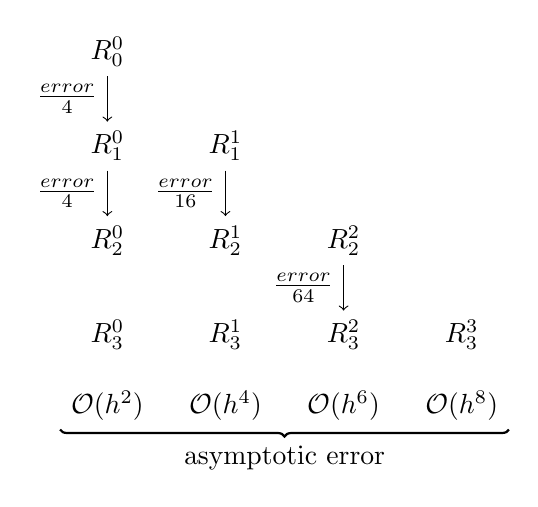
\begin{tikzpicture}[x=1.5cm,y=1.2cm]
            \node[] at (0, 0) (00) {$R^0_0$};
            \node[] at (0, -1) (01) {$R^0_1$};
            \node[] at (0, -2) (02) {$R^0_2$};
            \node[] at (0, -3) (03) {$R^0_3$};
            \node[] at (1, -1) (11) {$R^1_1$};
            \node[] at (1, -2) (12) {$R^1_2$};
            \node[] at (1, -3) (13) {$R^1_3$};
            \node[] at (2, -2) (22) {$R^2_2$};
            \node[] at (2, -3) (23) {$R^2_3$};
            \node[] at (3, -3) (33) {$R^3_3$};

            \draw [->] (00) -- node [midway, left] {$\frac{\text{error}}{4}$} (01);
            \draw [->] (01) -- node [midway, left] {$\frac{\text{error}}{4}$} (02);
            \draw [->] (11) -- node [midway, left] {$\frac{\text{error}}{16}$} (12);
            \draw [->] (22) -- node [midway, left] {$\frac{\text{error}}{64}$} (23);

            
            \node[] at (0, -3.75) () {$\mathcal{O}(h^2)$};
            \node[] at (1, -3.75) () {$\mathcal{O}(h^4)$};
            \node[] at (2, -3.75) () {$\mathcal{O}(h^6)$};
            \node[] at (3, -3.75) () {$\mathcal{O}(h^8)$};
            \draw [thick, decorate, decoration = {brace}] (3.4,-4) -- (-0.4,-4);
            \node[] at (1.5, -4.3) () {asymptotic error};
        \end{tikzpicture}
    \end{center}
\end{example}

\if 0
\begin{example}
Approximate $\int_1^3 \frac{1}{x} \,dx$ by trapezoid rule. How many subintervals
($n$) are needed to get $\text{error} < 10^{-2}$?
We use the theorem with the respective values:
\[
    \abs{\int_1^3 \frac{1}{x} \,dx - T\Bigl(\frac{1}{x}; P\Bigr)} = 
    \frac{1}{12} \cdot 2 \cdot h^2 \cdot \abs{f''(\xi)} \overset{!}{<} 10^{-2}
    \text{ for } \xi \in (1, 3)
\]
Find $h$ such that
\[
    \frac{1}{6} h^2 \abs{f''(\xi)} < 10^{-2}
\]
\end{example}
\fi